One crucial service in an operating system is its \emph{file system}, the
software that implements the abstraction of files and directories on top of a
disk, which simply stores a long sequence of bytes. File systems are important
because they are used by all applications to store data, and bugs in file
systems are especially costly because they can lead to data loss for any of
these applications. This thesis describes an approach towards building a
reliable and correct file system using formal verification, in which the file
system is developed along with a proof that it always follows a high-level
specification of its intended behavior. The artifact of this thesis is DaisyNFS,
a verified file system that comes with a proof of correctness and gets good
performance.

\section{Motivation}
\label{sec:intro:motivation}

A file system is an especially critical part of the systems software stack for
three reasons. First, the file system is widely used --- essentially all applications have
data that is ultimately stored in a file system. Second, implementations are
concurrent and optimized, which increases the potential for bugs. Finally, bugs
are particularly costly since they can lead to permanent data loss for any
application running on top.

Two challenges make implementing a correct file system challenging: crashes and
concurrency. A file system is generally expected to keep application data safe
even if the system stops running at any time, say due to a power failure or
kernel panic. This thesis uses ``crash'' to refer to any of these circumstances
where the computer stops and is rebooted. After a reboot, the file system is
expected to preserve data from before the crash. The second big challenge is
concurrency in the implementation, which complicates approaches for improving
reliability, including both testing and verification.

The approach in this thesis to make a reliable file system is to use formal
verification. In this approach, we write the code, then a specification of the
intended behavior of the code, and finally a mathematical proof that shows the
code always meets the specification. For confidence in the proof itself, the
proof is carried out in a computer and a piece of software called a proof
assistant checks that the proof is valid. The nature of formal verification
forces the proof engineer to systematically cover every corner case in the code.

While the idea of formal verification is not new, there was essentially no
support for reasoning about the combination of crashes and concurrency when this
thesis work started (in 2015). Thus this thesis develops new techniques to
reason about the combination in the first place. We apply these techniques to
DaisyNFS, a verified implementation of the Network File System (NFS) protocol, a
standard file-system interface.

The key to scaling up to a system with the complexity of DaisyNFS is a design
that splits the file system into two main parts: a transaction system called
GoTxn that makes it easy to get atomicity over the disk, and then the rest of
the file system implemented using a transaction per operation. GoTxn must face
the key challenges of crash safety and concurrency, but it handles them in such
a way that the code on top is verified using comparatively much simpler
sequential reasoning. The file-system code then focuses on implementing features
like the details of the NFS semantics, large files, and efficient data
structures.

\section{State of the art}
\label{sec:intro:related}

Production file systems are generally validated by testing. While testing is
indispensable for development, the nature of a file system makes it difficult to
catch all bugs with only testing. The fundamental difficulty is a high degree of
non-determinism from two sources: crashes in the middle of execution, and
concurrency in the implementation that is needed for good performance.

The importance of file-system correctness has been recognized by the academic
community, thus there are many approaches for increasing confidence with
improved testing. One line of work has explored systematically testing crashes
at intermediate points~\cite{mohan:crashmonkey,pillai:appcrash,yang:explode}. Another line of
work has focused on fuzz testing as a way to induce crash-safety
bugs~\cite{xu:janus,kim:hydra}. These approaches have been successful for
finding bugs, including crash-safety bugs, but they only test sequential
executions, missing bugs due to concurrently issued operations or from crashes
that interrupt multiple operations. Furthermore, unlike formal verification, testing cannot
cover all executions of a program, even without crashes and concurrency,
potentially missing bugs.

The research community has also recognized the value of formal verification for
reasoning about a file-system implementation. The closest related work is
another verified, concurrent file system,
Flashix~\cite{bodenmuller:concurrent-flashix}. Flashix runs on top of a
lower-level storage technology, raw flash rather than an SSD.\@ The techniques
developed to verify Flashix are specialized to its particular file-system
design, especially its write-back cache. Its concurrency is primarily between
regular operations and garbage collection, and read-only concurrency. DaisyNFS
has a different file-system design with write-write concurrency and a general
crash safety solution using transactions, whereas Flashix accounts for flash
failures and thus crashes in every write to storage.

There are other verified file systems, especially the sequential file systems
FSCQ~\cite{chen:fscq} and Yggdrasil~\cite{sigurbjarnarson:yggdrasil} and an
concurrent but in-memory file system AtomFS~\cite{zou:atomfs}. These systems use
verification techniques that do not support both crashes and concurrency, and we
cannot extend them in a straightforward way to support the other form of reasoning.

% \section{Challenges in implementing file systems}
%
% %% this section covered an unrelated concern, discussing how DaisyNFS provides
% %% the strongest crash safety and concurrency guarantees.
%
% Fundamentally a file system is a data structure that stores files inside a
% hierarchy of directories. That makes the implementation challenging is that the file system must persist all
% of its data into disk blocks, and we would like the file system to keep
% stored data safe even in the face of an interruption like a kernel panic,
% power failure, or sudden disconnect of the storage device. We call such an
% interruption a crash and use the term ``crash safety'' to refer to the goal of
% correctness even under crashes. Without appropriate care in the implementation,
% a naive implementation could lose or corrupt data. Data loss is particularly bad
% when
% metadata is corrupted --- for example, if a directory is moved by removing it
% from its original parent and then adding it to the new parent, interrupting this
% process might lose the directory and all of its contents.
%
% To get good performance, it is helpful to take advantage of multiple CPUs to
% prepare concurrent operations. However, this concurrency adds complexity on top
% of implementing the file system as a crash-safe data structure. Concurrency and
% storage also interact, since an efficient file system will improve performance
% by taking advantage of concurrently-issued writes to combine multiple disk
% operations into one.
%
% With both crash safety and concurrency, there is a wide spectrum of guarantees
% the file system might make about what happens with concurrent operations and
% crashes. The informal goal is for the system to never lose data, even when used concurrently. For the approach of this thesis, we need a more formal
% definition of correctness to prove that the system meets.
%
% Applications and users can have different expectations for what guarantees the
% file system makes. DaisyNFS implements the strongest guarantee for concurrency
% and crash safety: every operation should appear to occur at a single instant in
% time, or in other words should be atomic. This holds for concurrent threads as
% well as if a system crashes and the system reboots. Operations that are in
% progress might still be interrupted on crash, so data in the process of being
% written will be lost, but this is unavoidable if the system never reached the
% point of persisting that data.
%
% File systems do offer weaker guarantees --- especially allowing recently-written
% data to be lost on crash in order to defer writing data persistently
% --- but it is generally difficult to formalize and verify a system that provides
% these weaker guarantees. In any case the NFS specification requires most operations to be persistent
% when they return, restricting when an NFS server can take advantage
% of weaker durability guarantees. Instead of relaxing the guarantees we focused
% on a fairly efficient implementation of our strong atomic specification.

\section{Approach}
\label{sec:intro:approach}

What does it mean to give a machine checked, formal proof of a system? At a high
level, program proofs always have three components: an implementation, a
specification, and a proof. When doing machine-checked proofs, all three are
physically represented as code in a verification system. The verification system
checks the proof against the implementation and specification, ensuring that the
proof is complete.

This thesis integrates interactive, foundational proofs using custom
infrastructure (in Coq) as well as automated verification using a
verification-aware programming language (Dafny). These are both machine-checked,
formal proofs, but the interaction models of the two systems are different
enough that we explain them separately.

In Coq, the core feature is proofs based on dependent type theory, which is
expressive enough to represent essentially any math. A first step when using Coq
is to connect the code to the reasoning in the proof assistant. The approach in this thesis translates executable code to a model in Coq, but other approaches are possible. The model and its semantics encodes any
assumptions the proof makes about how the program behaves. The semantics is typically structured as a transition
system, where an execution is a sequence of states the program goes through
along with some notion of observable behavior, like external I/O or return
values.

Once we have a program in Coq, we can reason about it. The goal of
verification is to prove that the program meets its specification, and
where the specification describes the allowed behaviors of the program. The
specifications in this work forbid universally incorrect behavior, like reading an
out-of-bounds address in an array, but more precisely specify what the program
is supposed to do, for example how it responds to user requests.


A common structure to tame the complexity of reasoning about a program is to use
a \emph{program logic}. In principle it might be possible to prove a theorem
about all the behaviors of a program directly, but such a proof would too
complex to be feasible. The program logic organizes the proof with a structured
way of expressing and proving statements about the program, such as breaking the
proof down into theorems about individual functions. The proof in a program
logic will often mirror the structure of the code, since each function has its
own specification and groups of related functions have related specs.

Program logics for concurrency are still an active area of research; only
recently have they reached the maturity to give completely mechanized proofs of
moderate-sized programs. There are few logics that also can reason about crash
safety. Our approach in this thesis is to build a new program logic called Perennial with all the
concurrency-reasoning features of a modern program logic, plus new features for
reasoning about crashes. What makes this feasible is Iris, a modular framework
for concurrency. Iris includes a concurrent program logic which we are able to
extend with crash-safety reasoning while preserving the concurrency reasoning
features, without reimplementing them from scratch.

Using our new program logic, we verified GoTxn, a concurrent transaction system.
The transaction system's correctness theorem says that any program that uses
transactions really has transactional behavior: its execution is equivalent to a
version of the program where the transactions run atomically. The complete
specification includes some important details in order to formalize the
intuition behind atomicity.

Next, because transactions appear to run sequentially, and write to disk all at
once, it is no longer necessary to use a sophisticated program logic like
Perennial to reason about the body of each transaction. Instead, we switch to
using Dafny, a verification-oriented programming language that can only reason
about sequential code but as a result is highly productive for this kind of
software. The file system is written and verified in Dafny, then compiled to Go
and linked with GoTxn.

Dafny verification works quite differently from Coq. Dafny is a programming
language with verification features; contrast this with Coq, which supports
general math that can \emph{model} programs. A Dafny method can be annotated
with a specification. The Dafny checker converts a method and its specification
to a logical formula (called a verification condition), which is true if and only if the specification holds for
the method. It then queries a \emph{solver} (Z3, in the case of Dafny) to determine if the formula is true.
Contrast all of this with Coq, where the user manually develops the program
logic and connects the rules of this logic. Checking a program against its specification in Dafny cannot be perfectly
automated because it is impossible to answer whether a general logical formula
is true or not, but the user can insert annotations to help out the solver, and
generally fewer annotations are needed than lines of proof for Coq. The main
downside to this approach is that it fixes a sequential programming language, so
unlike in Coq, it isn't possible to reason about concurrency and crashes.

One of the contributions of this thesis is that the file-system design isolates
concurrency and crash safety into the transaction system. This structure leaves
the rest of the implementation only to \emph{sequentially} implement the
file-system logic and data structures. Because this is sequential, crash-free
execution, we use Dafny to implement and verify each operation, then run this
code wrapped in a transaction. Later we will have more to say about the file
system's proof, but for now suffice it to say that we show it correctly
implements the NFS protocol.

In order to connect the file system's sequential proofs to its concurrent
execution, we prove a general theorem about the transaction system's
implementation. The starting point is the idea of a \emph{simulation} proof,
which shows that a system like the file-system transactions correctly implement an
abstract specification like the NFS protocol. The GoTxn
\emph{simulation-transfer theorem} shows that for any system implemented using
transactions with a sequential simulation proof, the concurrent system running
with GoTxn concurrently simulates its abstract specification where each
operation is atomic. Intuitively this theorem holds because every concurrent
execution of the GoTxn transactions appears to be atomic, and then the
sequential simulation proof shows those atomic transactions implement the
abstract specification. However, the GoTxn theorem formalizes precisely what
conditions are required for the simulation transfer, including restrictions on
the transactions and exactly what crash safety guarantees are achieved.

\Cref{fig:overview} depicts how the artifacts of this thesis combine. GoTxn is
implemented in Go and verified using Perennial in Coq. Goose is the system that
connects the code to a model suitable for reasoning in Perennial. Separately,
DaisyNFS implements the file-system operations in Dafny, which has integrated
support for code and proofs. On the left-hand side of the figure,
\cc{daisy-nfsd} uses the verified code for DaisyNFS (compiled from Dafny to Go)
and GoTxn to implement a complete NFS server. On the right-hand side, the GoTxn
simulation transfer theorem takes the DaisyNFS Dafny proof and turns it into an
overall correctness theorem for the whole server.

\begin{figure}
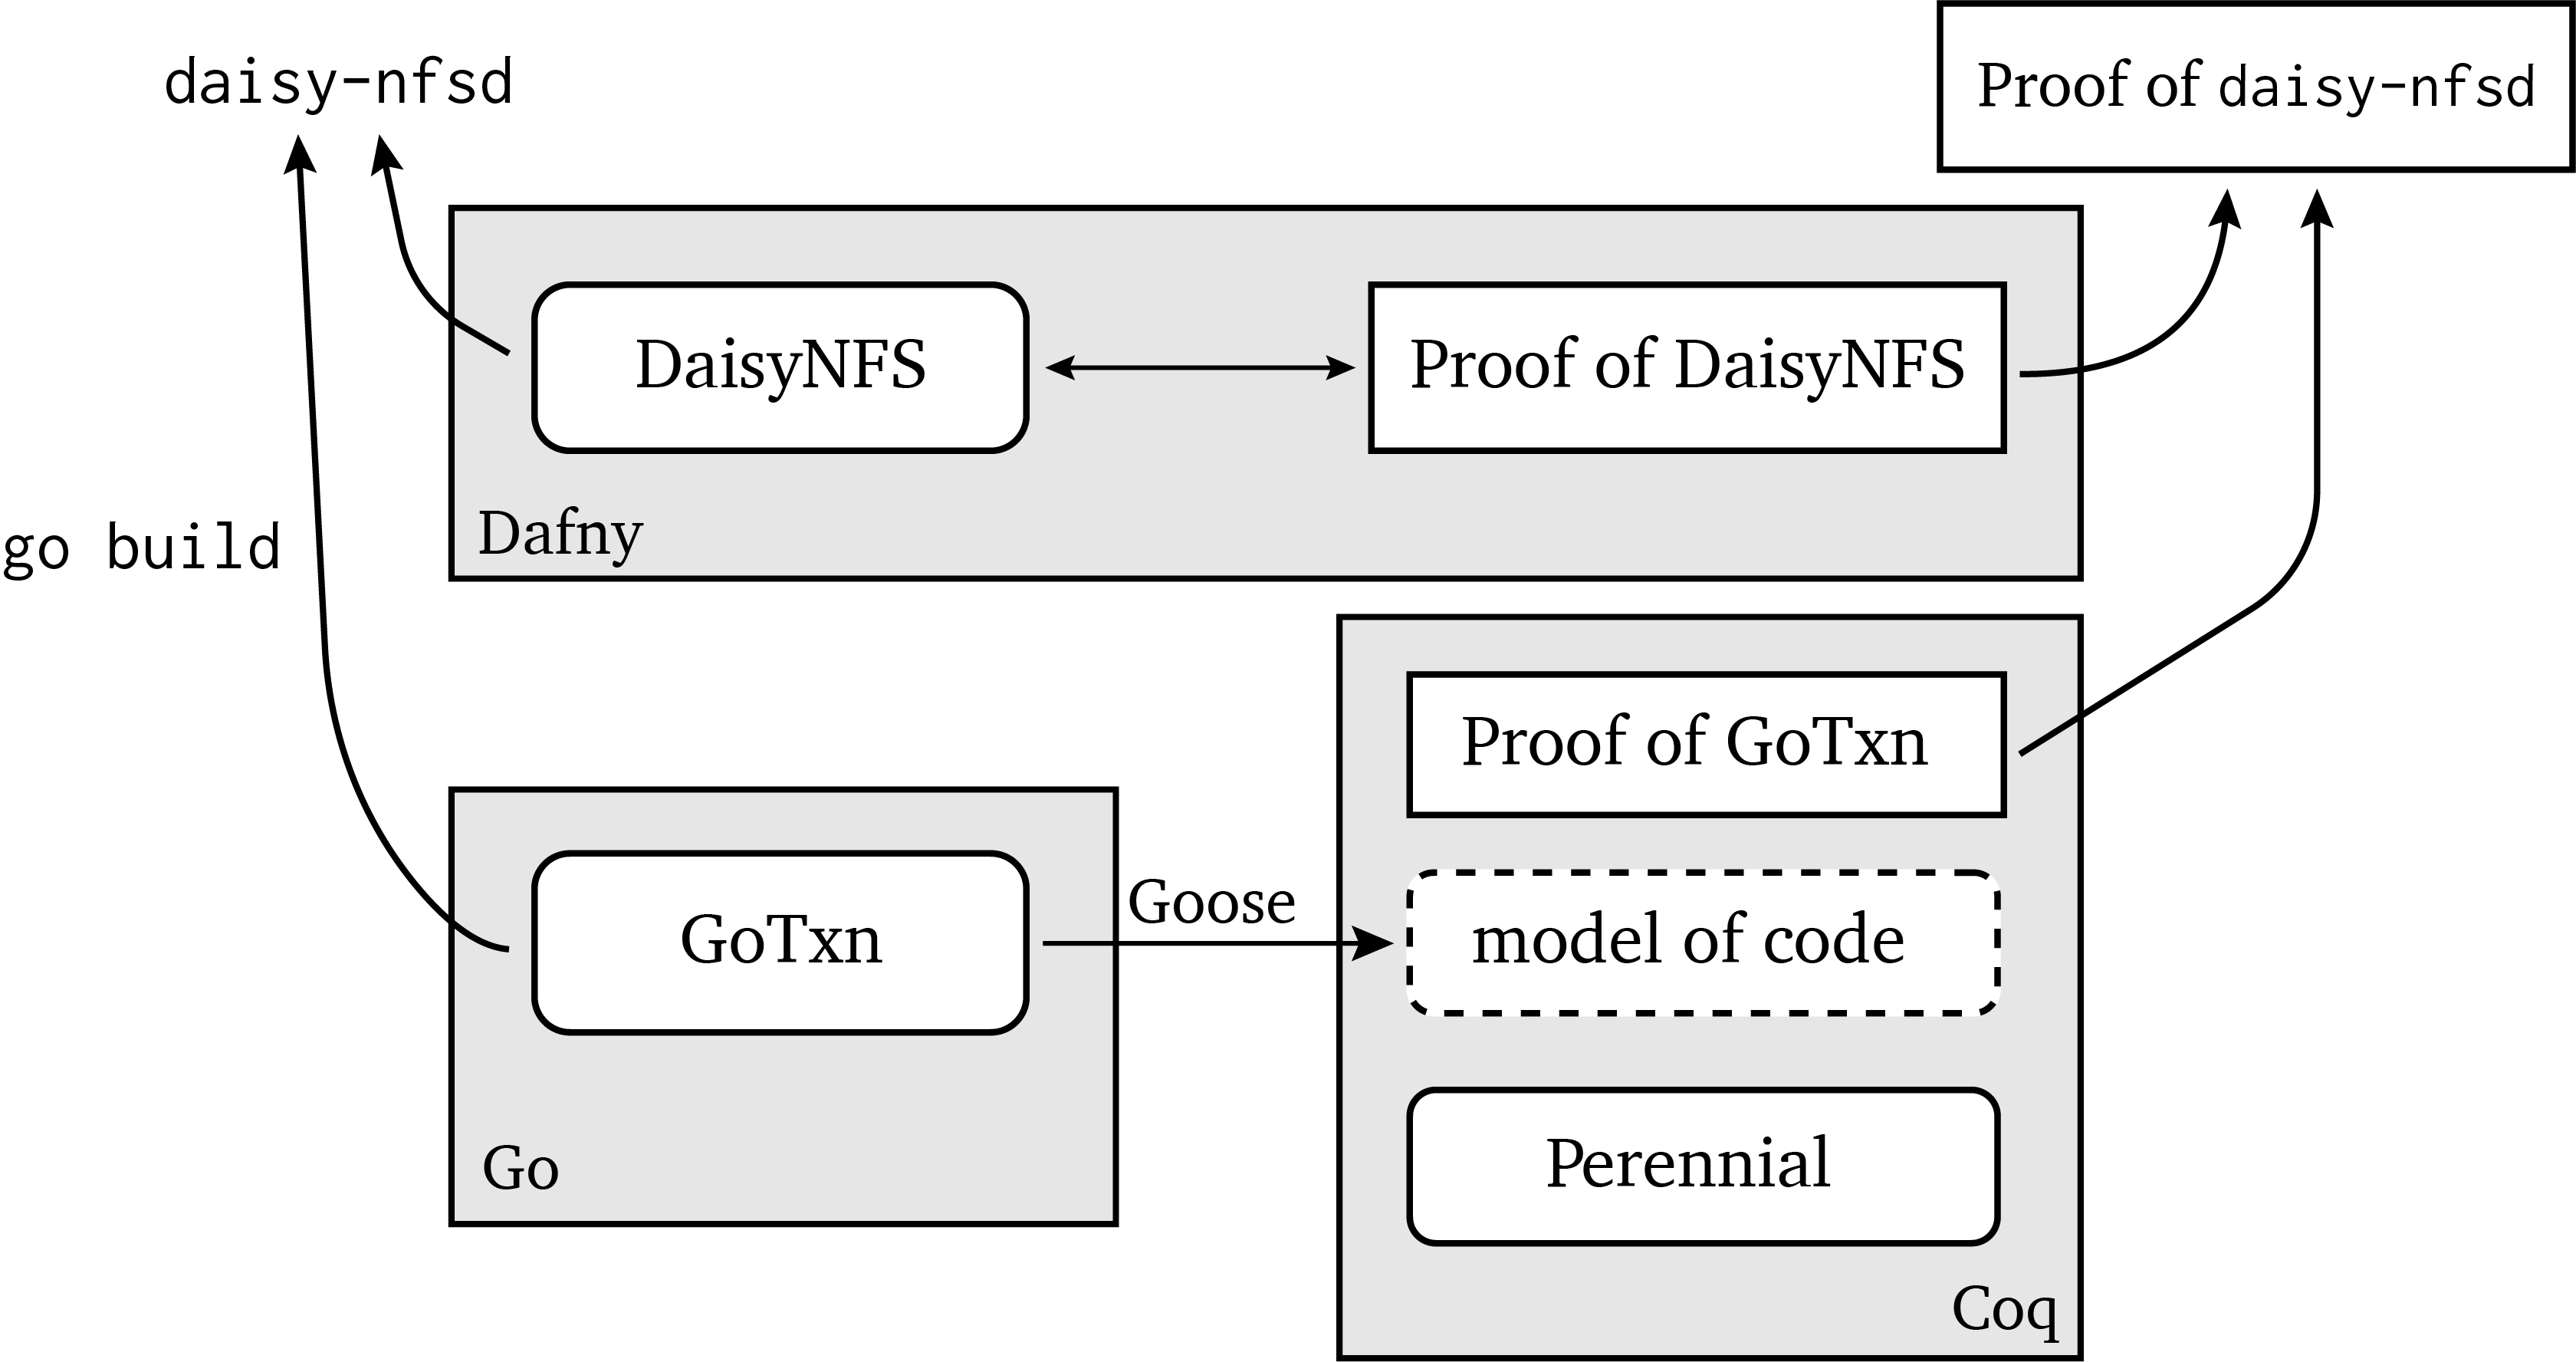
\includegraphics{fig/overview.png}
\caption{Overview of how GoTxn, DaisyNFS, and the proofs fit together.}
\label{fig:overview}
\end{figure}

\section{Contributions}
\label{sec:intro:contributions}

This thesis makes several contributions that enable its overall goal of a
verified, concurrent file system.

\begin{itemize}
  \item \textbf{Perennial} has new techniques for reasoning about crash safety
        and concurrency using specifications based on crash weakest
        preconditions. These include crash conditions combined with concurrency
        and reasoning principles for moving ownership to a recovery procedure
        following a crash. \textbf{Logically atomic crash specifications} are a
        pattern using Perennial's crash weakest preconditions for specifying
        libraries that have both concurrent behavior and involve persistent
        state. These are implemented using Perennial and used in the GoTxn
        proof.
  \item GoTxn has a new \textbf{lifting-based specification} for its journaling
        layer to reason about concurrent transactions separately, which is
        challenging since the logical disk can change during a transaction to a
        concurrently committed transaction. Its proof uses a novel
        \textbf{history-based abstract state} for the write-ahead log. This model allowed us to carry
        out a modular proof where the write-ahead logging library hides most of
        its internal complexity, simplifying reasoning about the rest of the GoTxn
        code that uses it. Finally, GoTxn exports a \textbf{program refinement}
        specification that captures how transactions appear to run atomically.
  \item DaisyNFS uses a \textbf{simulation-transfer theorem}, proven on top of
        GoTxn's program refinement specification, which shows that sequential
        reasoning for each transaction in a system implies correctness for the
        whole system when run on top of GoTxn. This justifies using Dafny, a
        sequential verification language, to verify the DaisyNFS implementation.
        The specification for DaisyNFS uses a mathematical formulation of RFC
        1813, the document that (in prose) specifies what a NFSv3 server should
        do.
  \item \textbf{Goose} connects efficient code implemented in Go to a model of
        that code in Perennial. A general contribution here is a design for
        systems verification that enables efficient code and convenient
        reasoning. Goose includes reasoning principles for the models that it
        outputs, to support verifying the translated code.
\end{itemize}

The ideas in Perennial and Goose are applied to GoTxn, but they could be used
for reasoning about other concurrent storage systems written in Go. Similarly,
this thesis applied GoTxn to a verified file system, but it could also be used
as the basis for other verified storage systems, like a persistent key-value
store.

\section{Reading guide for the thesis}
\label{sec:intro:reading-guide}

This section briefly outlines the chapters of the thesis, the dependencies
between chapters, and the intended audience. Broadly the thesis is intended for
a systems audience, except for the verification foundations. The support for
concurrency makes all of the formal underpinnings in the work more technical
than foundations for sequential systems verification.

\Cref{ch:related} covers related work across Perennial, GoTxn, and DaisyNFS, for
a broad computer-science audience. To keep the Goose chapter self-contained, its
related work is described in the relevant chapter.

\Cref{ch:perennial} is an overview of Perennial. This chapter is oriented
towards a reader interested in the general verification concepts and not
necessarily the systems side. At this level of abstraction Perennial is
independent of both the GoTxn proof and even Goose for verifying Go code. Some
experience with program logics is helpful for understanding the presentation.

\Cref{ch:crash-logatom} describes a style of logically atomic specifications
that capture both concurrency and crash atomicity using Perennial. It uses an
extended example from the GoTxn proof and explains its formal underpinnings at a
high level. This is the most technically involved chapter.

\Cref{ch:txn} describes the GoTxn proof. An important part of GoTxn is its
specification, which captures how transactions are atomic. This chapter does not
require the full Perennial or logical atomicity chapters.

\Cref{ch:daisy-nfs} describes the design and proof of DaisyNFS.\@ This chapter
explains the proof approach which justifies using Dafny to verify DaisyNFS even
though Dafny is a sequential verification tool and DaisyNFS is a concurrent
system.

\Cref{ch:goose} is about Goose and talks about verifying Go code generally, with
nothing specific to GoTxn or even storage systems. This is the first detailed
description of Goose, so this chapter is written to be readable without any of
the other chapters.

\Cref{ch:impl} is a short chapter covering some implementation details in
DaisyNFS, covering both GoTxn and the file-system code.

\Cref{ch:eval} evaluates the whole file system along a few dimensions,
especially performance but also aspects of the proof.
